\documentclass[pract]{SCWorks}
\usepackage{preamble}
\usepackage{siunitx}

\setminted{style=bw,
           linenos=true,
           breaklines=true,
           numbersep=5pt,
           tabsize=2,
           fontsize=\small,
           bgcolor=white}
\setmintedinline{style=bw,
                 bgcolor=white,
                 fontsize=\normalsize}

\begin{document}

% Кафедра (в родительном падеже)
\chair{математической кибернетики и компьютерных наук}

% Тема работы
\title{Тема работы}

% Курс
\course{2}

% Группа
\group{251}

% Факультет (в родительном падеже) (по умолчанию "факультета КНиИТ")
% \department{факультета КНиИТ}

% Специальность/направление код - наименование
% \napravlenie{02.03.02 "--- Фундаментальная информатика и информационные технологии}
% \napravlenie{02.03.01 "--- Математическое обеспечение и администрирование информационных систем}
% \napravlenie{09.03.01 "--- Информатика и вычислительная техника}
\napravlenie{09.03.04 "--- Программная инженерия}
% \napravlenie{10.05.01 "--- Компьютерная безопасность}

% Для студентки. Для работы студента следующая команда не нужна.
% \studenttitle{студентки}

% Фамилия, имя, отчество в родительном падеже
\author{Толстова Роберта Сергеевича}


% Кафедра (в родительном падеже)
\chair{математической кибернетики и компьютерных наук}
% Руководитель ДПП ПП для цифровой кафедры (перекрывает заведующего кафедры)
% \chpretitle{ заведующий кафедрой математических основ информатики и олимпиадного\\ программирования на базе МАОУ <<Ф"=Т лицей №1>>
% }
\chtitle{г. Саратов, к.\,ф.-м.\,н., доцент}
\chname{С.\,В.\,Миронов}

% Научный руководитель (для реферата преподаватель проверяющий работу)
\satitle{доцент, к.\,ф.-м.\,н.} %должность, степень, звание
\saname{М.\,И.\,Сафрончик}
\satitle{доцент, к.\,ф.-м.\,н.} %должность, степень, звание 

% Семестр (только для практики, для остальных типов работ не используется)
\term{1}

% Наименование практики (только для практики, для остальных типов работ не
% используется)
\practtype{учебная}

% Продолжительность практики (количество недель) (только для практики, для
% остальных типов работ не используется)
\duration{18}

% Даты начала и окончания практики (только для практики, для остальных типов
% работ не используется)
\practStart{02.09.24}
\practFinish{12.01.25}
% Тема работы
\title{Разработка приложений Windows.Forms на языке C++ в среде Microsoft Visual Studio}

% Курс
\course{2}

% Группа
\group{251}

% Руководитель практики от организации (руководитель для цифровой кафедры)
\patitle{доцент, к.\,ф.-м.\,н.}
\paname{М.\,И.\,Сафрончик}

% Семестр (только для практики, для остальных типов работ не используется)
\term{2}

% Наименование практики (только для практики, для остальных типов работ не
% используется)
\practtype{учебная}

% Продолжительность практики (количество недель) (только для практики, для
% остальных типов работ не используется)
\duration{2}

% Даты начала и окончания практики (только для практики, для остальных типов
% работ не используется)
\practStart{01.07.2024}
\practFinish{13.01.2024}

% Год выполнения отчета
\date{2024}

\maketitle

% Включение нумерации рисунков, формул и таблиц по разделам (по умолчанию -
% нумерация сквозная) (допускается оба вида нумерации)
\secNumbering

\tableofcontents

% Раздел "Обозначения и сокращения". Может отсутствовать в работе
% \abbreviations
% \begin{description}
%     \item ... "--- ...
%     \item ... "--- ...
% \end{description}

% Раздел "Определения". Может отсутствовать в работе
% \definitions

% Раздел "Определения, обозначения и сокращения". Может отсутствовать в работе.
% Если присутствует, то заменяет собой разделы "Обозначения и сокращения" и
% "Определения"
% \defabbr

\intro
Целью практики является освоение механизма построения оконных интерфейсов приложений на языке C++/CLI и фреймворках .NET и Windows Forms в среде Microsoft Visual Studio\cite{docs-vs-cpp-cli}.

В результате прохождения данной практики должны быть отработаны следующие навыки:

\begin{itemize}
    \item создание нового проекта;
    \item добавление и настройка пользовательских элементов управления;
    \item валидация пользовательского ввода;
    \item разработка алгоритма для решения поставленной задачи с использованием оконного интерфейса;
    \item тестирование приложений;
    \item документирование разработанного кода.
\end{itemize}

%\section{Вычисление факториала}
\subsection{Условие задания}
Разработать приложение для вычисления факториала по приведённому примеру.

Приложение должно содержать следующие компоненты:

\begin{enumerate}
  \item Заголовок формы должен отражать суть задания.
  \item Все элементы формы должны быть внятно подписаны (кнопки подписаны, у текстового поля должно быть написано, для чего оно нужно и т.д.)
  \item В коде должны быть комментарии и отступы (код должен быть легко читаем).
  \item В коде программы все элементы формы должны быть переименованы (btnName -  для кнопок, lblName - для ссылок, txtName - для текстового поля и т. д.) Наименования должны быть понятными.
  \item Приложение должно корректно работать (выводить ответ или ошибку с соответствующим сообщением) для следующих данных: ввод буквы, ввод отрицательного числа, ввод нуля, ввод положительного числа (< 10), ввод большого положительного числа. После вывода ошибок при вводе корректных данных поля ошибок должны очищаться.
\end{enumerate}

\subsection{Факториал натурального числа}
Факториалом натурального числа $n$ называют число $n!$, такое, что:

\begin{equation}
  n! = 1 \times 2 \times \dots \times (n - 1) \times n
\end{equation}

\subsection{Нахождение факториала рекурсивным способом}
Пусть на вход подано число $n\in\mathbb{N}$. Тогда алгоритм \cite{factorial-calculation} будет выглядеть таким образом:
\begin{itemize}
  \item Если $0 \leqslant n \leqslant 1$, то возвращаем $0! = 1! = 1$;
  \item Если $n > 1$, то возвращаем $n! = (n-1)!\times n$.
\end{itemize}
Таким образом, мы можем рекурсивно вычислить факториал любого достаточно малого числа $n$. Для больших чисел алгоритм будет медленным в силу экстремально быстрого роста функции факториала.

\subsection{Вид формы в конструкторе}
Форма имеет вид:
\begin{figure}
  \centering
  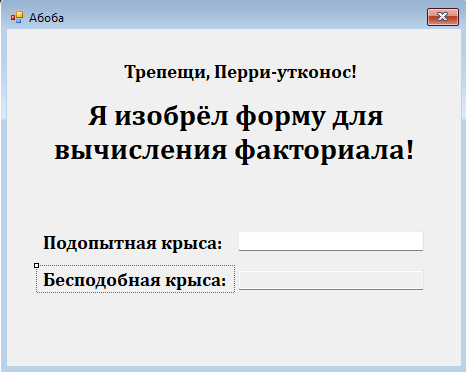
\includegraphics[width=0.5\linewidth]{images/factorial/form.png}
  \caption{Форма окна для вычисления факториала}
  \label{fig:factorial-form}
\end{figure}

\subsection{Таблица с описанием элементов формы}
Все элементы формы были переименованы для большей читаемости. В таблице \ref{tab:factorial-form} представлены все изменения.

\begin{table}
  \centering
  \begin{tabular}{|m{0.3\textwidth}|m{0.3\textwidth}|m{0.3\textwidth}|}
    \hline
    \textbf{Описание элементов формы} & \textbf{Список изменённых атрибутов} & \textbf{Новое значение атрибута} \\
    \hline
    \hline
    Окно формы & Text & Абоба \\
    Верхний подзаголовок & Name & lblSubtitle \\
    Верхний заголовок & Name & lblTitleStart \\
    Нижний заголовок & Name & lblTitleEnd \\
    Метка поля ввода & Name & lblInput \\
    Метка поля вывода & Name & lblOutput \\
    Поле ввода & Name & textInput \\
    Поле вывода & Name & textOutput \\
    \hline
  \end{tabular}
  \caption{Значение атрибутов элементов в приложении для вычисления факториала}
  \label{tab:factorial-form}
\end{table}

\subsection{Примеры правильной и неправильной работы приложения}
При запуске приложения на экране появляется окно \ref{fig:factorial-start}.
\begin{figure}
  \centering
  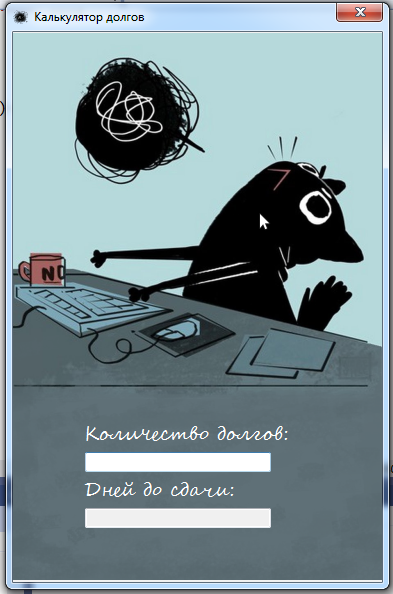
\includegraphics[width=0.5\linewidth]{images/factorial/start.png}
  \caption{Запуск программы}
  \label{fig:factorial-start}
\end{figure}

При вводе реактивно подсчитывается и подставляется значение в поле вывода. Также реактивно происходит обработка ошибок.

\begin{figure}
  \centering
  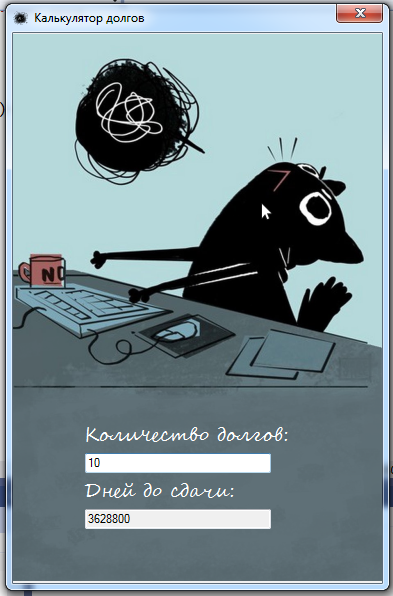
\includegraphics[width=0.5\linewidth]{images/factorial/okay.png}
  \caption{Запуск программы с корректными данными}
  \label{fig:factorial-okay}
\end{figure}

\begin{figure}
  \centering
  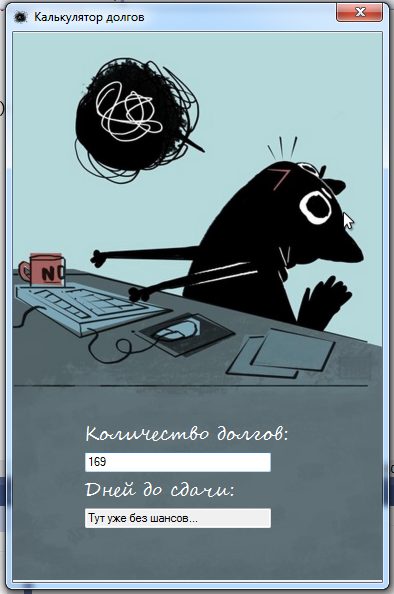
\includegraphics[width=0.5\linewidth]{images/factorial/error.png}
  \caption{Запуск программы с некорректными числовыми данными}
  \label{fig:factorial-error}
\end{figure}

\begin{figure}
  \centering
  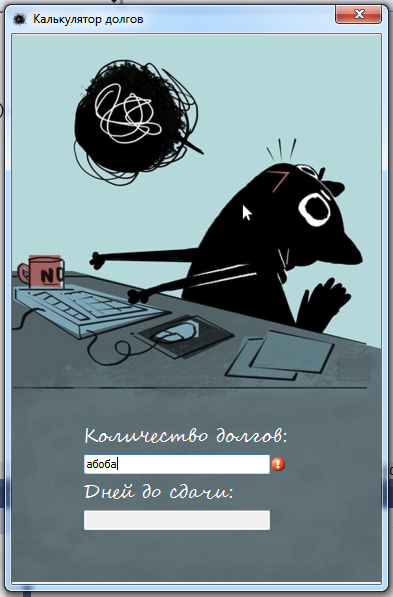
\includegraphics[width=0.5\linewidth]{images/factorial/error2.png}
  \caption{Запуск программы с нечисловыми данными}
  \label{fig:factorial-error2}
\end{figure}

\subsection{Примеры исходного кода}
\begin{minted}{cpp}
/* Процедура для очистки экрана */
private: void ClearAll() {
  this->textOutput->Text = "";
  errorProvider->SetError(textInput, String::Empty);
}

/* Обработчик события изменения текстового поля */
private: System::Void textInput_onChange(System::Object^ sender, System::EventArgs^ e) {
  ClearAll();
  long long InputNumber;
  bool result = Int64::TryParse(this->textInput->Text, InputNumber);

  // в result записали булеву переменную, отвечающую за корректный ввод
  if (!result)
    errorProvider->SetError(textInput, "Введено не целое число");
  else {
    // по условию задачи число не должно быть больше 20
    if (InputNumber > 20)
      this->textOutput->Text = "Слишком большое число";
    else {
      // внешняя рекурсивная функция факториала вернёт -1 только в одном случае -- если исходное число отрицательное
      long long OutputNumber = factorial(InputNumber);
      if (OutputNumber == -1)
        errorProvider->SetError(textInput, "Введено отрицательное число");
      else this->textOutput->Text = System::Convert::ToString(OutputNumber);
    }
  }
}
\end{minted}

Больше кода проекта доступно в приложении \ref{application-A}. Также в приложенном архиве можно найти полный код проекта.
%\section{Простые вычисления}
\subsection{Условие задания}
Выполнить задание. Номер варианта --- 8.

Выражение:
\begin{equation}
\frac{\cos{2x^2} + \sin^2{y}}{x + y} + yx
\end{equation}

Проверить работу созданного приложения на приведенных тестовых примерах. Тесты сделаны на Visual Studio 2008, поэтому обращайте внимание только на первые шесть цифр после запятой.

Приложение должно содержать следующие компоненты:

\begin{enumerate}
\item Заголовок формы должен отражать суть задания.
\item Все элементы формы должны быть внятно подписаны (кнопки подписаны, у тестового поля должно быть написано, для чего оно нужно и т. д.)
\item В коде должны быть комментарии и отступы (код должен быть легко читаем).
\item Должна быть проверка ошибок - ввод не числа, ввод числа, находящегося за пределами ОДЗ, ввод числа, принадлежащего ОДЗ.
\item Если надо ввести 2 значения, то в случае ввод букв в оба поля, ошибка должна быть у обоих полей; в случае ввода одной буквы - только у того поля, где буква.
\end{enumerate}

\subsection{Основы тригонометрии}
В Евклидовой геометрии синусом угла называют отношение противолежащего этому углу катета к гипотенузе. Косинус угла --- отношение прилежащего к этому углу катета к гипотенузе.

Математический анализ обобщает эти функции на всю числовую прямую, делая их периодическими с периодом $2\pi$.

Таким образом $\forall x \in \mathbb{R}\; \exists \sin{x}, \cos{x} \in \mathbb{R}$.

\subsection{Нахождение значений функций синуса и косинуса}
Для нахождения значений выражений мы воспользуемся встроенной в C++ библиотекой cmath.

\subsection{Вид формы в конструкторе}
Форма имеет вид:

\begin{figure}
\centering
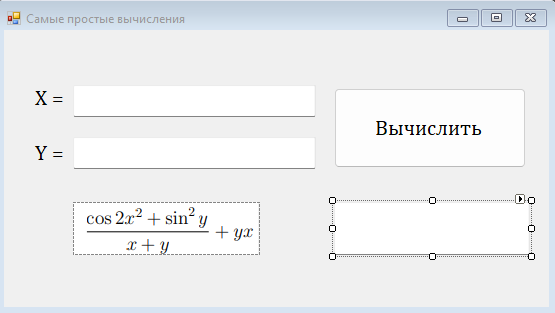
\includegraphics[width=0.5\linewidth]{images/simple-calculations/form.png}
\caption{Форма окна для задания <<Простые вычисления>>}
\label{simple-calculations-form}
\end{figure}

\subsection{Таблица с описанием элементов формы}
Все элементы формы были переименованы для большей читаемости. В таблице \ref{tab:simple-calculations-form} представлены все изменения.

\begin{table}
\centering
\begin{tabular}{|m{0.3\textwidth}|m{0.3\textwidth}|m{0.3\textwidth}|}
\hline
\textbf{Описание элементов формы} & \textbf{Список изменённых атрибутов} & \textbf{Новое значение атрибута} \\
\hline
\hline
Окно формы & Text & Самые простые вычисления \\
Метка для X & Name & xLabel\\
Метка для Y & Name & yLabel \\
Поле для ввода X & Name & xTextbox \\
Поле для ввода Y & Name & yTextbox \\
Поле для вывода & Name & outputTextbox \\
Поле для выражения PictureBox & Name & expressionPicturebox \\
Кнопка <<Вычислить>> & Name & calculateButton \\
\hline
\end{tabular}
\caption{Значение атрибутов элементов в приложении для простых вычислений}
\label{tab:simple-calculations-form}
\end{table}

\subsection{Примеры правильной и неправильной работы приложения}
При запуске приложения на экране появляется окно \ref{fig:simple-calculations-start}.

\begin{figure}
\centering
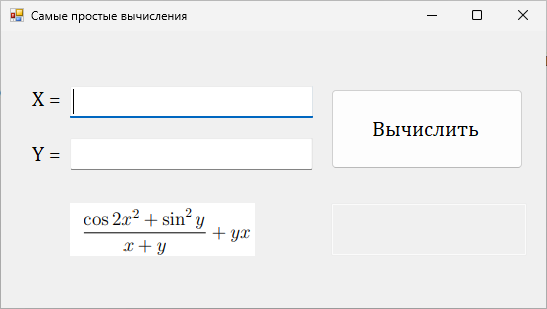
\includegraphics[width=0.5\linewidth]{images//simple-calculations/start.png}
\caption{Запуск программы}
\label{fig:simple-calculations-start}
\end{figure}

При нажатии на кнопку подсчитывается и подставляется значение в поле вывода. Также происходит обработка ошибок.

\begin{figure}
\centering
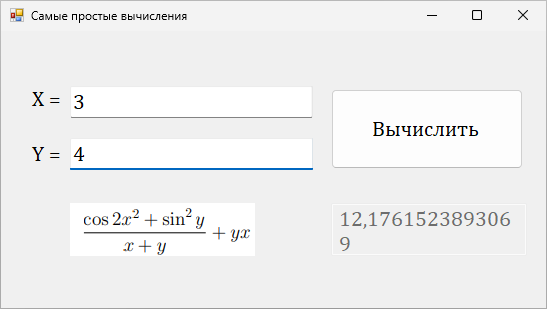
\includegraphics[width=0.5\linewidth]{images//simple-calculations/okay.png}
\caption{Запуск с корректными данными}
\label{fig:simple-calculations-okay}
\end{figure}

\begin{figure}
\centering
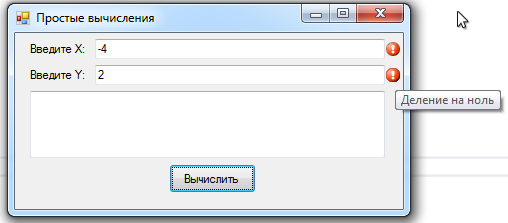
\includegraphics[width=0.5\linewidth]{images//simple-calculations/error.png}
\caption{Пример ввода с программно корректными, но математически некорректными данными}
\label{fig:simple-calculations-error}
\end{figure}

\begin{figure}
\centering
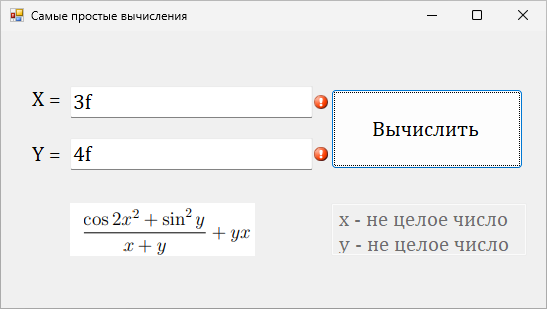
\includegraphics[width=0.5\linewidth]{images//simple-calculations/error2.png}
\caption{Пример ввода с программно некорректными данными}
\label{fig:simple-calculations-error2}
\end{figure}

\subsection{Примеры исходного кода}
\begin{minted}{cpp}
/* процедура для очистки всех полей ввода и ошибок */
private: System::Void ClearAll() {
    this->outputTextbox->Text = "";
    this->errorProvider->Clear();
}

/* бизнес-логика: вычисление выражения */
private: double CalculateExpression(int x, int y) {
if (x + y == 0) {
    throw gcnew DivideByZeroException();
    return 0;
}

    return((cos(2 * x * x) + pow(sin(y), 2)) / (x + y)) + (y * x);
}

/* обработка события нажатия на кнопку <<Вычислить>> */
private: System::Void calculateButton_Click(System::Object^ sender, System::EventArgs^ e) {
    ClearAll();
    
    String^ rawX = gcnew String(this->xTextbox->Text);
    String^ rawY = gcnew String(this->yTextbox->Text);
    String^ error = "";
    
    int x, y;
    
    if (!Int32::TryParse(rawX, x)) {
        error += "x - не целое число";
        this->errorProvider->SetError(this->xTextbox, "x - не целое число");
    }

    if (!Int32::TryParse(rawY, y)) {
        if (error->Length != 0) {
            // если сообщений об ошибках несколько, то разделим их символом \n
            error += Environment::NewLine;
        }
        error += "y - не целое число";
        this->errorProvider->SetError(this->yTextbox, "y - не целое число");
    }

    if (error->Length != 0) {
      this->outputTextbox->Text = error;
      return; // нет смысла обрабатывать некорректные данные
    }

    double result;
    try {
      result = CalculateExpression(x, y);
    }
    catch (DivideByZeroException^ e) {
      this->outputTextbox->Text = "Деление на ноль";
      return;
    }

    this->outputTextbox->Text = Convert::ToString(result);
}
\end{minted}

Больше кода проекта доступно в приложении \ref{application-A}. Также в приложенном архиве можно найти полный код проекта.
%\section{Рекурсивные вычисления}
\subsection{Условие задания}
Выполнить задание. Номер варианта --- 4.

Создать рекурсивную функцию, вычисляющую значение полинома Эрмита:
\begin{equation}
\begin{cases}
     H_0(x) = 1,\\
     H_1(x) = 2x,\\
     H_n(x) = 2x \times H_{n-1}(x) - 2n \times H_{n-2}(x).\\
\end{cases}
\end{equation}

Проверить работу созданного приложения на приведённых тестовых примерах. 

Приложение должно содержать следующие компоненты:
\begin{enumerate}
\item Заголовок формы должен отражать суть задания.
\item Все элементы формы должны быть внятно подписаны (кнопки подписаны, у тестового поля должно быть написано, для чего оно нужно и т. д.)
\item В коде должны быть комментарии и отступы (код должен быть легко читаем).
\item В коде программы все элементы формы должны быть переименованы (btnName -  для кнопок, lblName - для ссылок, txtName - для текстового поля и т. д.) Наименования должны быть понятными.
\item Приложение должно корректно работать (выводить ответ или ошибку с соответствующим сообщением) для следующих данных: ввод буквы, ввод отрицательного числа, ввод нуля, ввод положительного числа (< 10), ввод большого положительного числа. После вывода ошибок при вводе корректных данных поля ошибок должны очищаться.
\end{enumerate}

\subsection{Вид формы в конструкторе}
Форма имеет вид:

\begin{figure}
\centering
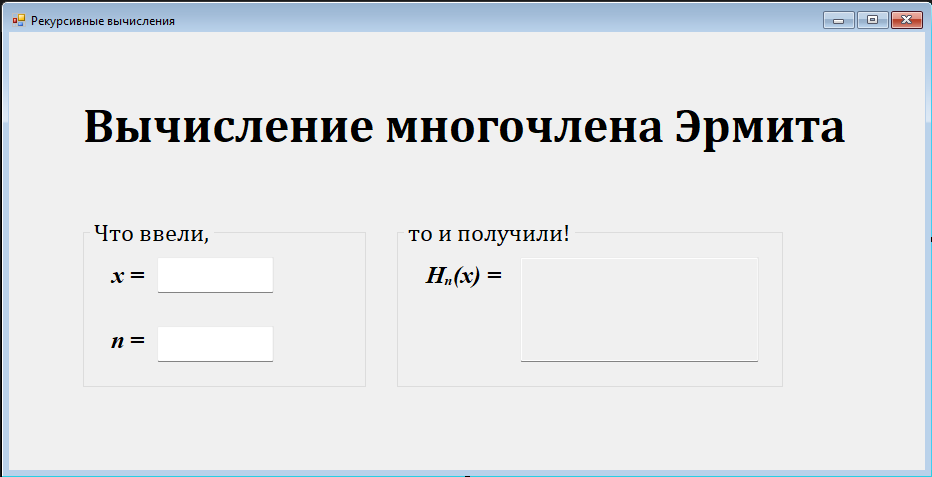
\includegraphics[width=0.5\linewidth]{images/recursive-calculations/form.png}
\caption{Форма окна для задания <<Рекурсивные вычисления>>}
\label{recursive-calculations-form}
\end{figure}

\subsection{Таблица с описанием элементов формы}
Все элементы формы были переименованы для большей читаемости. В таблице \ref{tab:recursive-calculations-form} представлены все изменения.

\begin{table}
\centering
\begin{tabular}{|m{0.3\textwidth}|m{0.3\textwidth}|m{0.3\textwidth}|}
\hline
\textbf{Описание элементов формы} & \textbf{Список изменённых атрибутов} & \textbf{Новое значение атрибута} \\
\hline
\hline
Окно формы & Text & Рекурсивные вычисления \\
Заголовок & Name & mainTitle \\
Группа ввода & Name & inputGroup \\
Группа вывода & Name & outputGroup \\
Метка для X & Name & xLabel \\
Метка для N & Name & nLabel \\
Поле ввода для X & Name & xTextBox \\
Поле ввода для N & Name & nTextBox \\
Метка для значения многочлена & Name & outputLabel \\
Поле вывода для значения многочлена & Name & outputTextBox \\
\hline
\end{tabular}
\caption{Значение атрибутов элементов в приложении для рекурсивных вычислений}
\label{tab:recursive-calculations-form}
\end{table}

\subsection{Примеры правильной и неправильной работы приложения}
При запуске приложения на экране появляется окно \ref{fig:recursive-calculations-start}.

\begin{figure}
\centering
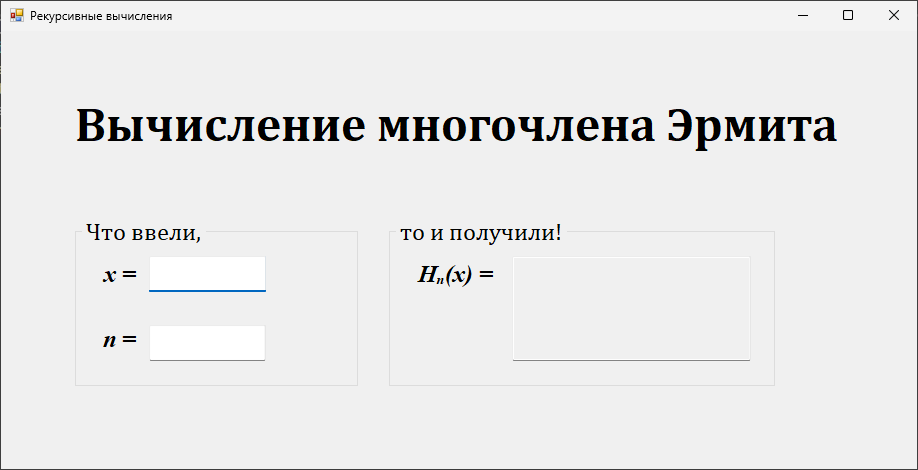
\includegraphics[width=0.5\linewidth]{images//recursive-calculations/start.png}
\caption{Запуск программы}
\label{fig:recursive-calculations-start}
\end{figure}

При изменении полей ввода реактивно подсчитывается и подставляется значение в поле вывода. Также происходит обработка ошибок.

\begin{figure}
\centering
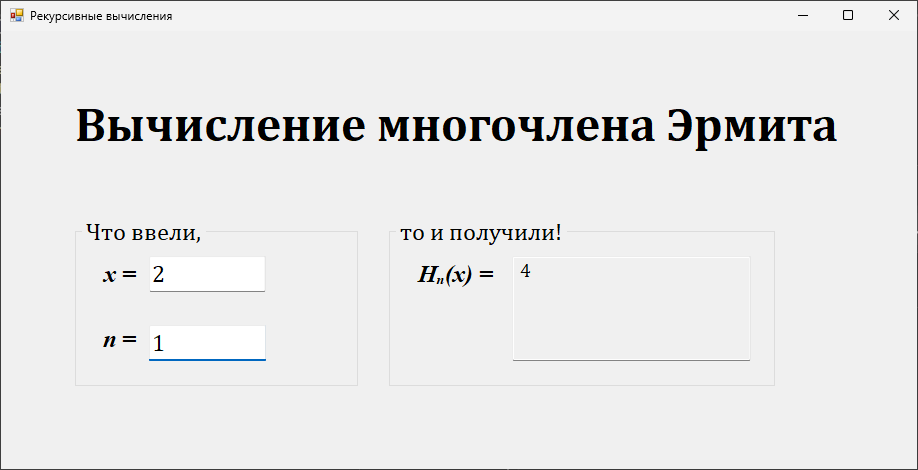
\includegraphics[width=0.5\linewidth]{images//recursive-calculations/okay.png}
\caption{Запуск с корректными данными}
\label{fig:recursive-calculations-okay}
\end{figure}

\begin{figure}
\centering
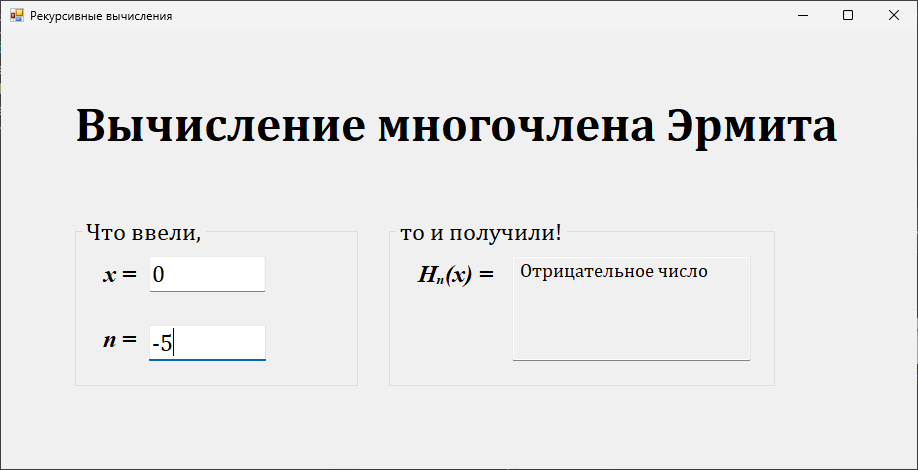
\includegraphics[width=0.5\linewidth]{images//recursive-calculations/error.png}
\caption{Пример ввода с некорректными данными}
\label{fig:recursive-calculations-error}
\end{figure}

\begin{figure}
\centering
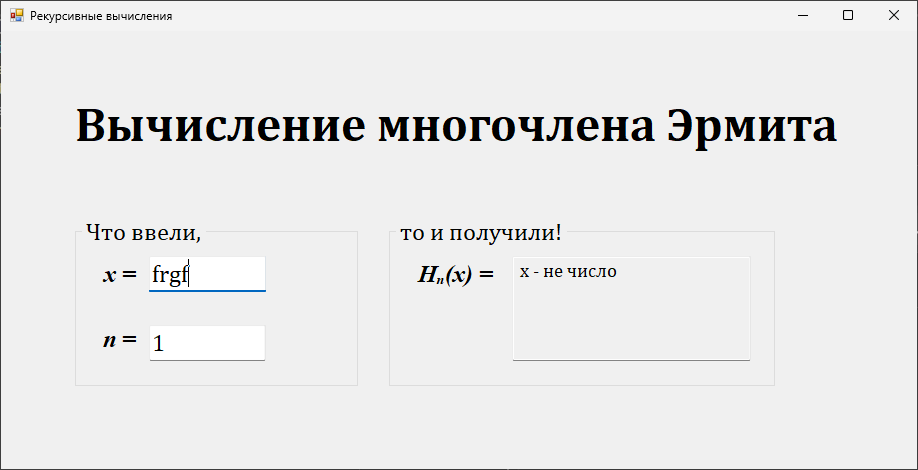
\includegraphics[width=0.5\linewidth]{images//recursive-calculations/error2.png}
\caption{Пример ввода с некорректными данными}
\label{fig:recursive-calculations-error2}
\end{figure}

\subsection{Примеры исходного кода}
\begin{minted}{cpp}
/* бизнес-логика для вычисления многочлена */
double H(long long n, double x) {
    if (n == 0) return 1.0;
    if (n == 1) return 2 * x;
    return (2 * x * H(n - 1, x) - 2 * n * H(n - 2, x));
}

/* обработка события изменения полей */
private: System::Void updateResult_TextBox(System::Object^ sender, System::EventArgs^ e) {
    double xInput = 0;
    bool resultX = Double::TryParse(this->xTextBox->Text, xInput);
    
    long long nInput = 0;
    bool resultN = Int64::TryParse(this->nTextBox->Text, nInput);
    
    if (!resultX && !resultN) {
        this->outputTextBox->Text = "x - не число, n - не целое число";
    }
    else if (!resultX) {
        this->outputTextBox->Text = "x - не число";
    }
    else if (!resultN) {
        this->outputTextBox->Text = "n - не целое число";
    }
    else if (nInput < 0) {
        this->outputTextBox->Text = "Отрицательное число";
    }
    else {
        this->outputTextBox->Text = System::Convert::ToString(H(nInput, xInput));
    }
}
\end{minted}

Больше кода проекта доступно в приложении \ref{application-A}. Также в приложенном архиве можно найти полный код проекта.
%\section{Обработка табличных данных. Часть 1}
\subsection{Условие задания}
Выполнить задание. Вариант: <<Найти сумму нечетных элементов с чётными порядковыми номерами. Вывести номера минимальных четных элементов>>.

Создать приложение для выполнения задания. Использовать элемент формы DataGridView. Диапазон $[a,b]$ означает, что $mas[i][j] >= a$ и $mas[i][j] <= b$

Приложение должно выполнять следующие действия:

\begin{enumerate}
\item Возможность удалять и добавлять строки таблицы. Проект не должен аварийно завершаться при удалении несуществующей таблицы.
\item Проверять ввод не числовых данных как в таблицу, так и в остальные текстовые поля (если есть в задании).
\item Если есть диапазон значений $[a,b]$, проверять, что $a < b$.
\item Заголовок формы должен отражать суть задания.
\item Все элементы формы должны быть внятно подписаны (кнопки подписаны, у тестового поля должно быть написано, для чего оно нужно и т. д.)
\item В коде должны быть комментарии и отступы (код должен быть легко читаем).
\item В коде программы все элементы формы должны быть переименованы (btnName -  для кнопок, lblName - для ссылок, txtName - для текстового поля и т.д.) Наименования должны быть понятными.
\item Приложение должно корректно работать (выводить ответ или ошибку с соответствующим сообщением). После вывода ошибок при вводе корректных данных поля ошибок должны очищаться.  
\end{enumerate}

\subsection{Вид формы в конструкторе}
Форма имеет вид:

\begin{figure}
\centering
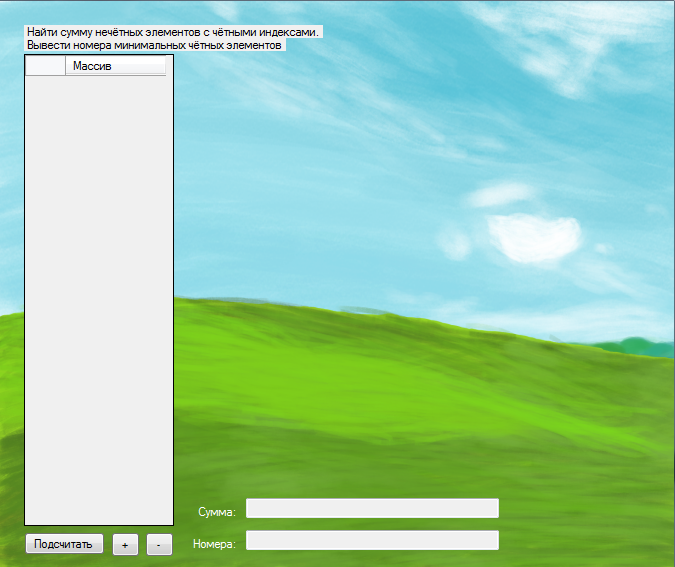
\includegraphics[width=0.5\linewidth]{images/handling-data-easy/form.png}
\caption{Форма окна для задания <<Простые вычисления>>}
\label{handling-data-easy-form}
\end{figure}

\subsection{Таблица с описанием элементов формы}
Все элементы формы были переименованы для большей читаемости. В таблице \ref{tab:handling-data-easy-form} представлены все изменения.

\begin{table}
\centering
\begin{tabular}{|m{0.3\textwidth}|m{0.3\textwidth}|m{0.3\textwidth}|}
\hline
\textbf{Описание элементов формы} & \textbf{Список изменённых атрибутов} & \textbf{Новое значение атрибута} \\
\hline
\hline
Окно формы & Text & Обработка табличных данных \\
Верхняя метка заголовка & Name & taskLabel \\
Нижняя метка заголовка & Name & taskLabel2 \\
Таблица & Name & arrayGridView \\
Кнопка <<Подсчитать>> & Name & countButton \\
Кнопка <<Добавить элемент>> & Name & addButton \\
Кнопка <<Удалить последний элемент>> & Name & popButton \\
Метка <<Сумма>> & Name & sumOddLabel \\
Метка <<Номера>> & Name & minsLabel \\
Поле для суммы & Name & outputOddSumTextBox \\
Поле для номеров & Name & outputMinsTextBox \\

\hline
\end{tabular}
\caption{Значение атрибутов элементов в приложении для обработки табличных данных}
\label{tab:handling-data-easy-form}
\end{table}

\subsection{Примеры правильной и неправильной работы приложения}
При запуске приложения на экране появляется окно \ref{fig:handling-data-easy-start}.

\begin{figure}
\centering
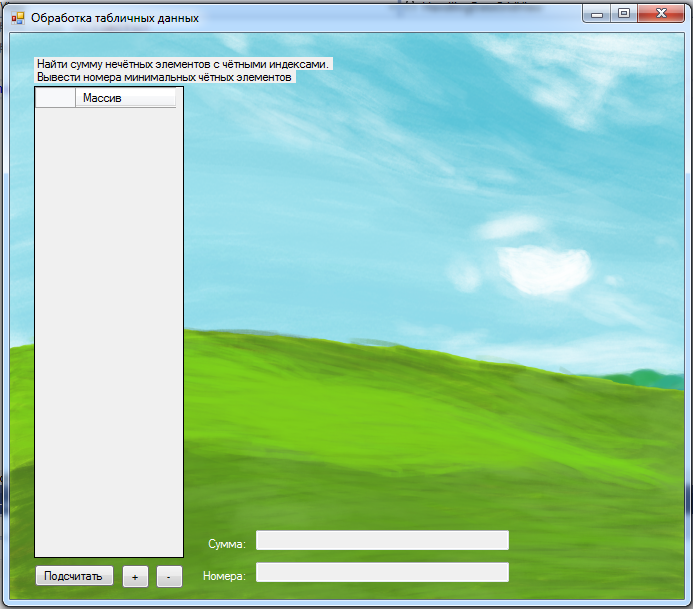
\includegraphics[width=0.5\linewidth]{images//handling-data-easy/start.png}
\caption{Запуск программы}
\label{fig:handling-data-easy-start}
\end{figure}

При нажатии на кнопку подсчитываются и подставляются значения в поля вывода. Также происходит обработка ошибок.

\begin{figure}
\centering
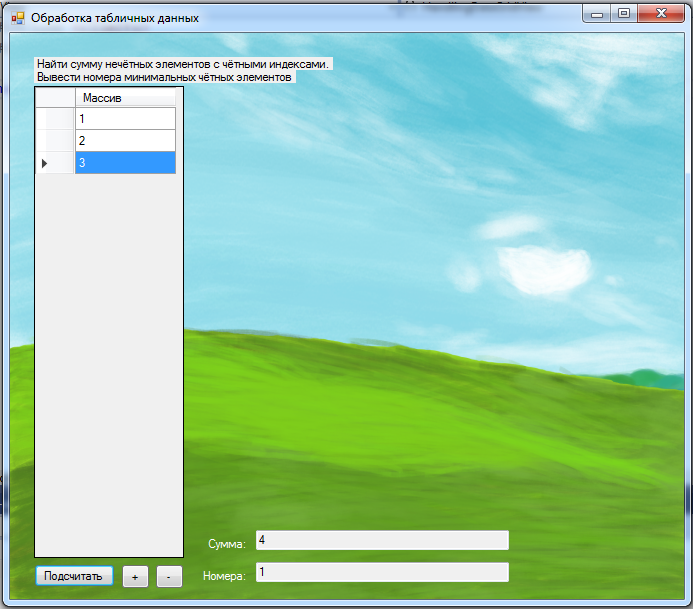
\includegraphics[width=0.5\linewidth]{images//handling-data-easy/okay.png}
\caption{Запуск с корректными данными}
\label{fig:handling-data-easy-okay}
\end{figure}

\begin{figure}
\centering
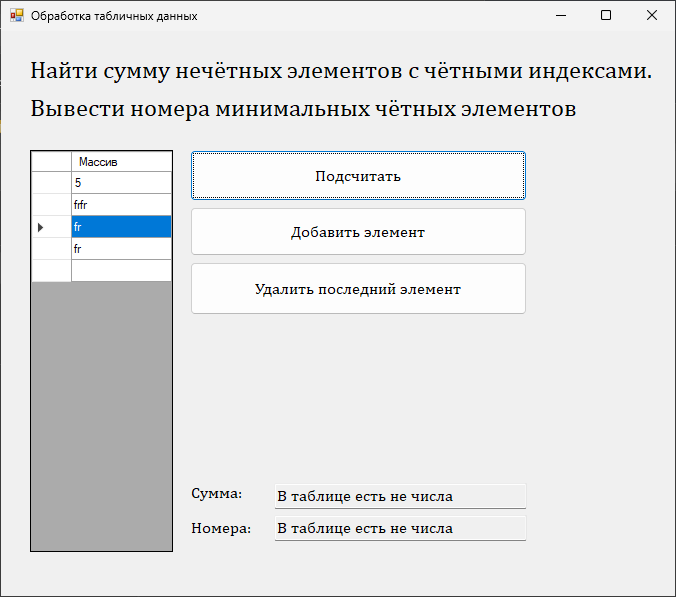
\includegraphics[width=0.5\linewidth]{images//handling-data-easy/error.png}
\caption{Пример ввода с некорректными данными}
\label{fig:handling-data-easy-error}
\end{figure}

\begin{figure}
\centering
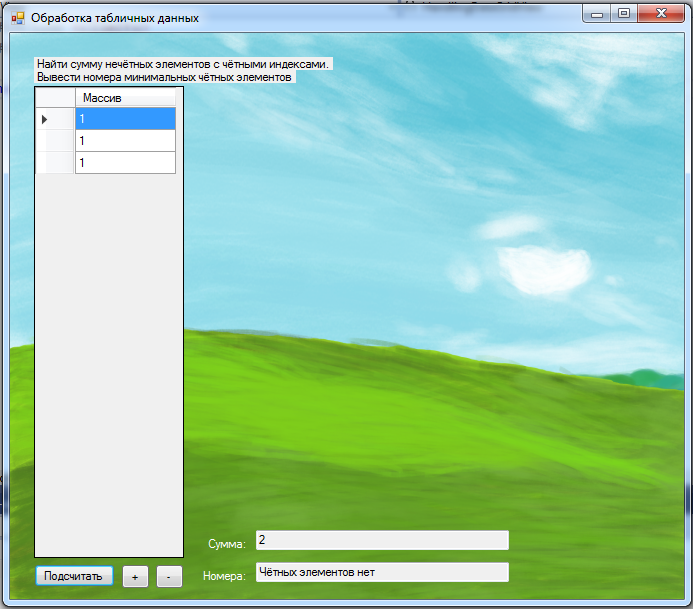
\includegraphics[width=0.5\linewidth]{images//handling-data-easy/error2.png}
\caption{Пример ввода с некорректными данными}
\label{fig:handling-data-easy-error2}
\end{figure}

\begin{figure}
\centering
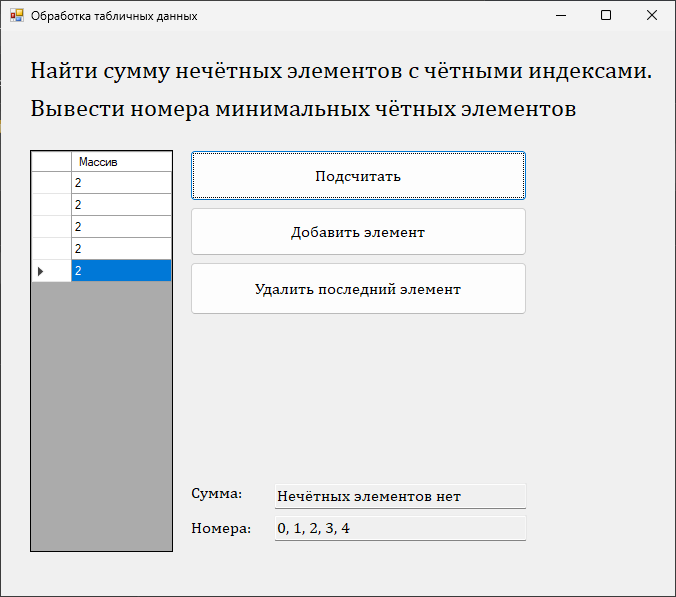
\includegraphics[width=0.5\linewidth]{images//handling-data-easy/error3.png}
\caption{Пример ввода с некорректными данными}
\label{fig:handling-data-easy-error3}
\end{figure}

\subsection{Примеры исходного кода}
\begin{minted}{cpp}
	/* функция для обновления вывода */
	private: OutputState^ GetOutput() {
		long long sum = 0;
		long long minEl = LLONG_MAX;

		String^ columnName = "Массив";
		OutputState^ state = gcnew OutputState();

		bool oddsFound = false;
		bool ifSummable = false;
		bool evensFound = false;

		for (int i = 0; i < this->arrayGridView->RowCount; ++i) {
			long long val;
			Object^ cellValue = this->arrayGridView->Rows[i]->Cells[columnName]->Value;

			if (cellValue == nullptr) {
				continue;
			}
			try {
				val = Convert::ToInt64(cellValue);
				if (val % 2 != 0 && i % 2 == 0) {
					sum += Convert::ToInt64(cellValue);
					ifSummable = true;
					oddsFound = true;
				}
				else if (val % 2 != 0) oddsFound = true;
				else {
					evensFound = true;
					if (val < minEl) {
						minEl = val;
						state->resultIdx = Convert::ToString(i);
					}
					else if (val == minEl) {
						state->resultIdx += ", " + Convert::ToString(i);
					}
				}
			}
			catch (FormatException^ e) {
				state->resultSum = "Разрешены только целые числа";
				state->resultIdx = state->resultSum;
				return state;
			}
		}

		state->resultSum = Convert::ToString(sum);
		if (!oddsFound) {
			state->resultSum = "Нечётных элементов нет";
		}
		else if (!ifSummable) {
			state->resultSum = "На чётных индексах нет нечётных";
		}
		if (!evensFound) {
			state->resultIdx = "Чётных элементов нет";
		}
		return state;
	}
\end{minted}

Больше кода проекта доступно в приложении \ref{application-A}. Также в приложенном архиве можно найти полный код проекта.
%\section{Обработка табличных данных. Часть 2}
\subsection{Условие задания}
Выполнить задание. Вариант: <<Заменить столбцы, содержащие только чётные элементы, столбцом X.>>.

Создать приложение для выполнения задания. Использовать элемент формы DataGridView. Диапазон $[a,b]$ означает, что $mas[i][j] >= a$ и $mas[i][j] <= b$

Приложение должно выполнять следующие действия:

\begin{enumerate}
\item Возможность удалять и добавлять строки таблицы. Проект не должен аварийно завершаться при удалении несуществующей таблицы.
\item Проверять ввод не числовых данных как в таблицу, так и в остальные текстовые поля (если есть в задании).
\item Если есть диапазон значений $[a,b]$, проверять, что $a < b$.
\item Заголовок формы должен отражать суть задания.
\item Все элементы формы должны быть внятно подписаны (кнопки подписаны, у тестового поля должно быть написано, для чего оно нужно и т. д.)
\item В коде должны быть комментарии и отступы (код должен быть легко читаем).
\item В коде программы все элементы формы должны быть переименованы (btnName -  для кнопок, lblName - для ссылок, txtName - для текстового поля и т.д.) Наименования должны быть понятными.
\item Приложение должно корректно работать (выводить ответ или ошибку с соответствующим сообщением). После вывода ошибок при вводе корректных данных поля ошибок должны очищаться.  
\end{enumerate}

\subsection{Вид формы в конструкторе}
Форма имеет вид:

\begin{figure}
\centering
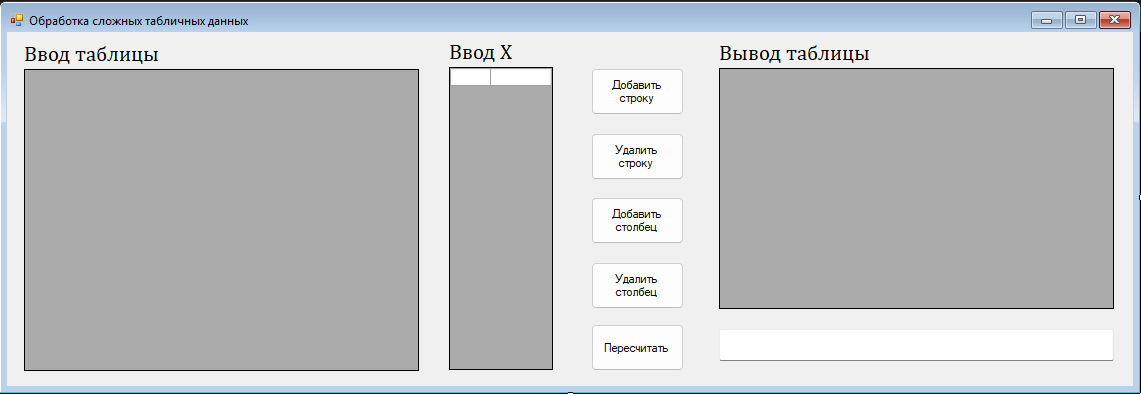
\includegraphics[width=0.5\linewidth]{images/handling-data-hard/form.png}
\caption{Форма окна для задания <<Простые вычисления>>}
\label{handling-data-hard-form}
\end{figure}

\subsection{Таблица с описанием элементов формы}
Все элементы формы были переименованы для большей читаемости. В таблице \ref{tab:handling-data-hard-form} представлены все изменения.

\begin{table}
\centering
\begin{tabular}{|m{0.3\textwidth}|m{0.3\textwidth}|m{0.3\textwidth}|}
\hline
\textbf{Описание элементов формы} & \textbf{Список изменённых атрибутов} & \textbf{Новое значение атрибута} \\
\hline
\hline
Окно формы & Text & Обработка сложных табличных данных \\
Метка <<Ввод таблицы>> & Name & tableInputLabel \\
Метка <<Ввод X>> & Name & xInputLabel \\
Метка <<Вывод таблицы>> & Name & outputLabel \\
Основная таблица ввода & Name & tableGrid \\
Дополнительная таблица ввода & Name & xGrid \\
Таблица вывода & Name & outputGridView \\
Поле для ошибок & Name & errorProvider \\
Кнопка <<Добавить строку>> & Name & addRow \\
Кнопка <<Удалить строку>> & Name & removeRow \\
Кнопка <<Добавить столбец>> & Name & addColumn \\
Кнопка <<Удалить столбец>> & Name & removeColumn \\
Кнопка <<Пересчитать>> & Name & executeButton \\

\hline
\end{tabular}
\caption{Значение атрибутов элементов в приложении для обработки табличных данных}
\label{tab:handling-data-hard-form}
\end{table}

\subsection{Примеры правильной и неправильной работы приложения}
При запуске приложения на экране появляется окно \ref{fig:handling-data-hard-start}.

\begin{figure}
\centering
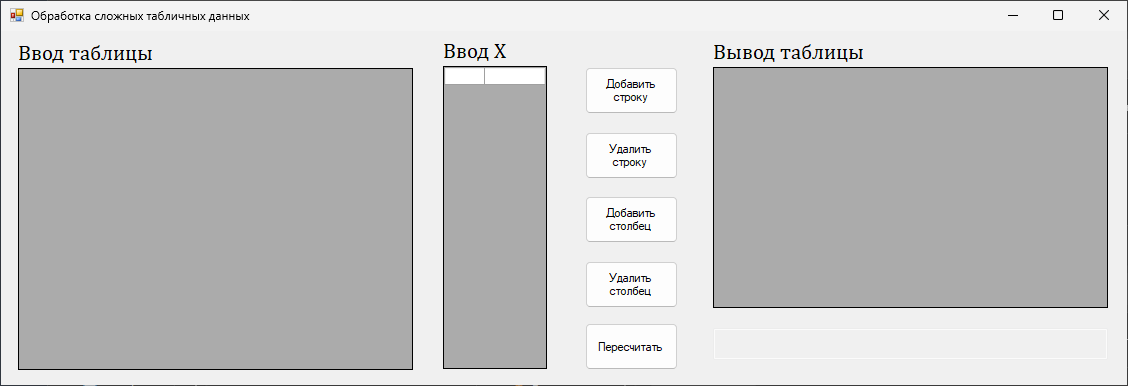
\includegraphics[width=0.5\linewidth]{images//handling-data-hard/start.png}
\caption{Запуск программы}
\label{fig:handling-data-hard-start}
\end{figure}

При нажатии на кнопку подсчитываются и подставляются значения в таблицу вывода. Также происходит обработка ошибок.

\begin{figure}
\centering
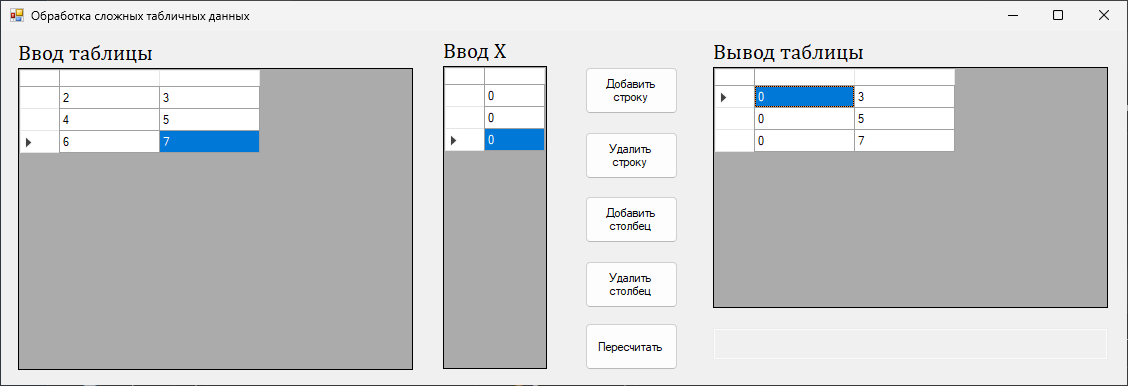
\includegraphics[width=0.5\linewidth]{images//handling-data-hard/okay.png}
\caption{Запуск с корректными данными}
\label{fig:handling-data-hard-okay}
\end{figure}

\begin{figure}
\centering
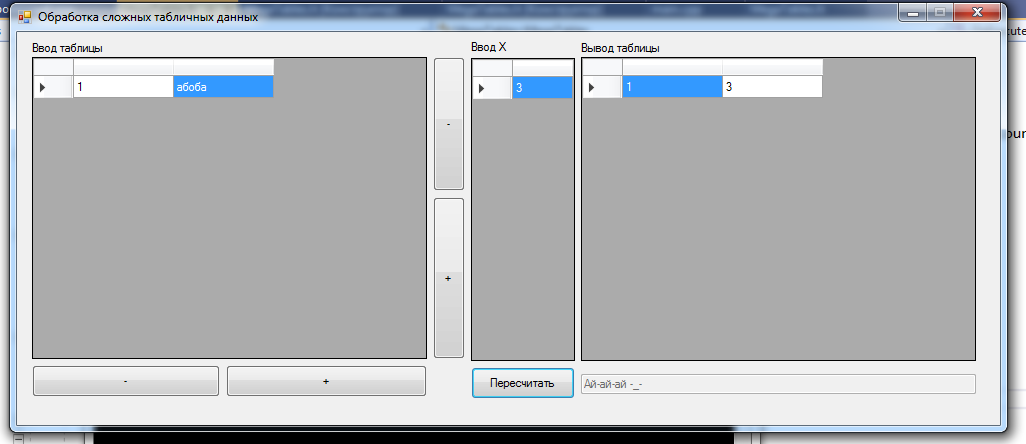
\includegraphics[width=0.5\linewidth]{images//handling-data-hard/error.png}
\caption{Пример ввода с некорректными данными}
\label{fig:handling-data-hard-error}
\end{figure}

\begin{figure}
\centering
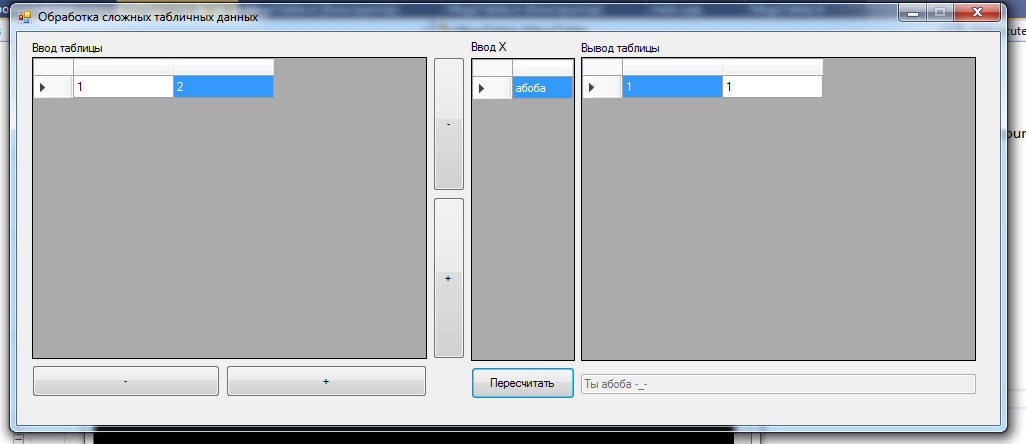
\includegraphics[width=0.5\linewidth]{images//handling-data-hard/error2.png}
\caption{Пример ввода с некорректными данными}
\label{fig:handling-data-hard-error2}
\end{figure}

\subsection{Примеры исходного кода}
\begin{minted}{cpp}
/* функция для обсчёта массива данных */
private: System::Void executeButton_Click(System::Object^ sender, System::EventArgs^ e) {
    int evenColumns = 0;
    try {
        for (int j = 0; j < this->tableGrid->Columns->Count; ++j) {
            bool flag = true;
            for (int i = 0; i < this->tableGrid->Rows->Count; ++i) {
                int value;
                Int32::TryParse(System::Convert::ToString(this->tableGrid->Rows[tableGrid->RowCount - i - 1]->Cells[j]->Value), value);
                if (value % 2 != 0) {
                    flag = false;
                    break;
                }
            }
    
            evenColumns++;
            for (int i = 0; i < this->tableGrid->Rows->Count; ++i) {
                if (flag) {
                    this->outputGridView->Rows[tableGrid->RowCount - i - 1]->Cells[j]->Value = this->xGrid->Rows[tableGrid->RowCount - i - 1]->Cells[0]->Value;
                }
                else {
                    this->outputGridView->Rows[tableGrid->RowCount - i - 1]->Cells[j]->Value = this->tableGrid->Rows[tableGrid->RowCount - i - 1]->Cells[j]->Value;
                }
    
            }
        }
    
        if (!evenColumns) {
            this->errorProvider->Text = "Нет чётных столбцов";
        }
    }
    catch (...) {
        this->errorProvider->Text = "Не удалось заменить столбцы";
    }
}
\end{minted}

Больше кода проекта доступно в приложении \ref{application-A}. Также в приложенном архиве можно найти полный код проекта.
\section{Матричный калькулятор}
\subsection{Условие задания}
Создать приложение,  реализующее основные операции с векторами и матрицами:

\begin{enumerate}
    \item Ввод матрицы, вектора;
    \item Создание матриц (единичная, матрица как набор векторов);
    \item Умножение на число, вектор, матрицу;
    \item Сложение/вычитание двух матриц;
    \item Сложение/вычитание двух векторов;
    \item Скалярное и векторное произведение двух векторов;
    \item Транспонированная матрица;
    \item Определитель, ранг матрицы.
\end{enumerate}

Выводить сообщения об ошибках (ввод не числа, несоответствие размерностей)

\subsection{Теория}
Вектором\cite{linal} называется направленный отрезок, для которого указаны его начало и конец. Свободный вектор --- множество одинаково направленных отрезков.

С точки зрения алгебры, вектор --- это строка или столбец матрицы.

Далее рассмотрим бинарные операции над векторами размерности $n \in \mathbb{N}$:
\begin{equation}
    \label{eq:vectors}
    \Vec{a} = \left(a_1, a_2, \dots, a_n\right),\;
    \Vec{b} = \left(b_1, b_2, \dots, b_n\right).
\end{equation}

Алгебраической суммой векторов (\ref{eq:vectors}) называют вектор:
\begin{equation}
    \Vec{a}+\Vec{b} = \left(a_1 + b_1, a_2 + b_2, \dots, a_n + b_n\right).
\end{equation}

Произведением вектора $\Vec{a}$ (\ref{eq:vectors}) на число $\lambda \in \mathbb{R}$ называют вектор:
\begin{equation}
    \lambda\Vec{a} = \left(\lambda a_1, \lambda a_2, \dots, \lambda a_n\right).
\end{equation}

Скалярным произведением векторов $\Vec{a} \cdot \Vec{b}$ (\ref{eq:vectors}) называют число:
\begin{equation}
    \Vec{a} \cdot \Vec{b} = \left|\Vec{a}\right|\left|\Vec{b}\right|\cos\angle\left(\Vec{a},\,\Vec{b}\right).
\end{equation}

Пусть $n = 3$ для векторов (\ref{eq:vectors}) --- из курса элементарной математики известно, что векторное произведение работает только в трёхмерном пространстве. Положим также, что векторы $\Vec{a}$ и $\Vec{b}$ не коллинеарны, то есть:
\begin{equation*}
    \exists\,i \in \mathbb{N}\cap\left[1,\,n\right]\;\forall\,\lambda\in\mathbb{N}\;a_i \neq \lambda b_i
\end{equation*}

Тогда векторным произведением называют вектор $\Vec{c}$ такой, что:
\begin{equation*}
    \begin{cases}
        \left|\Vec{c}\,\right| = S_{\Vec{a}\Vec{b}}, \\
        \Vec{c} \perp \Vec{a}, \\
        \Vec{c} \perp \Vec{b}, \\
        \left(\Vec{a},\,\Vec{b},\,\Vec{c}\right) - \textrm{правая тройка,}
    \end{cases}
\end{equation*}
где $S_{\Vec{a}\Vec{b}}$ --- площадь параллелограмма, построенного на $\Vec{a}$ и $\Vec{b}$ как на сторонах.

Матрицей называют прямоугольную таблицу чисел.

Далее рассмотрим матрицы:
\begin{equation}
    \label{eq:matrix}
    A = \begin{pmatrix} a_1^1 & \cdots & a_1^n \\ \vdots & \ddots & \vdots \\ a_n^1 & \cdots & a_n^n \\ \end{pmatrix},\;
    B = \begin{pmatrix} a_1^1 & \cdots & a_1^n \\ \vdots & \ddots & \vdots \\ a_m^1 & \cdots & a_m^n \\ \end{pmatrix},
\end{equation}
где $m,n\,\in\mathbb{N}$.

Матрицы вида $A$ (\ref{eq:matrix}) называют квадратными.

Пусть $i\,\in\mathbb{N}$ --- номер некоторой строки. Определителем квадратной матрицы называют число
\begin{equation}
    \left|A\right| = \det A = \begin{vmatrix} a_1^1 & \cdots & a_1^n \\ \vdots & \ddots & \vdots \\ a_n^1 & \cdots & a_n^n \\ \end{vmatrix}
    = \sum\limits_{k=1}^n\left(-1\right)^{k+i}a_i^kM_i^k,
\end{equation}
где $M_i^k$ -- определитель минора по элементу $A_i^k$. Это матрица, получаемая из исходной вычеркиванием строк и столбцов, содержащих $a_i^k$.

Определитель можно вычислить рекурсивно, сводя к базовому случаю $n=2$:
\begin{equation}
    \left|A\right| = \det A = \begin{vmatrix} a_1^1 & a_1^2 \\ a_2^1 & a_2^2 \\ \end{vmatrix}
    = a_1^1a_2^2 - a_1^2a_2^1,
\end{equation}

Ранг матрицы --- наивысший порядок среди порядков миноров этой матрицы, отличный от нуля. Вычисление ранга матрицы возможно методом Гаусса, что и было применено в программе.

Транспонированная матрица --- матрица со строками-столбцами и столбцами-строками исходной матрицы.

Алгебраическая сумма матриц определяется аналогичным векторам образом.

\subsection{Вид формы в конструкторе}
Форма имеет вид:

\begin{figure}
\centering
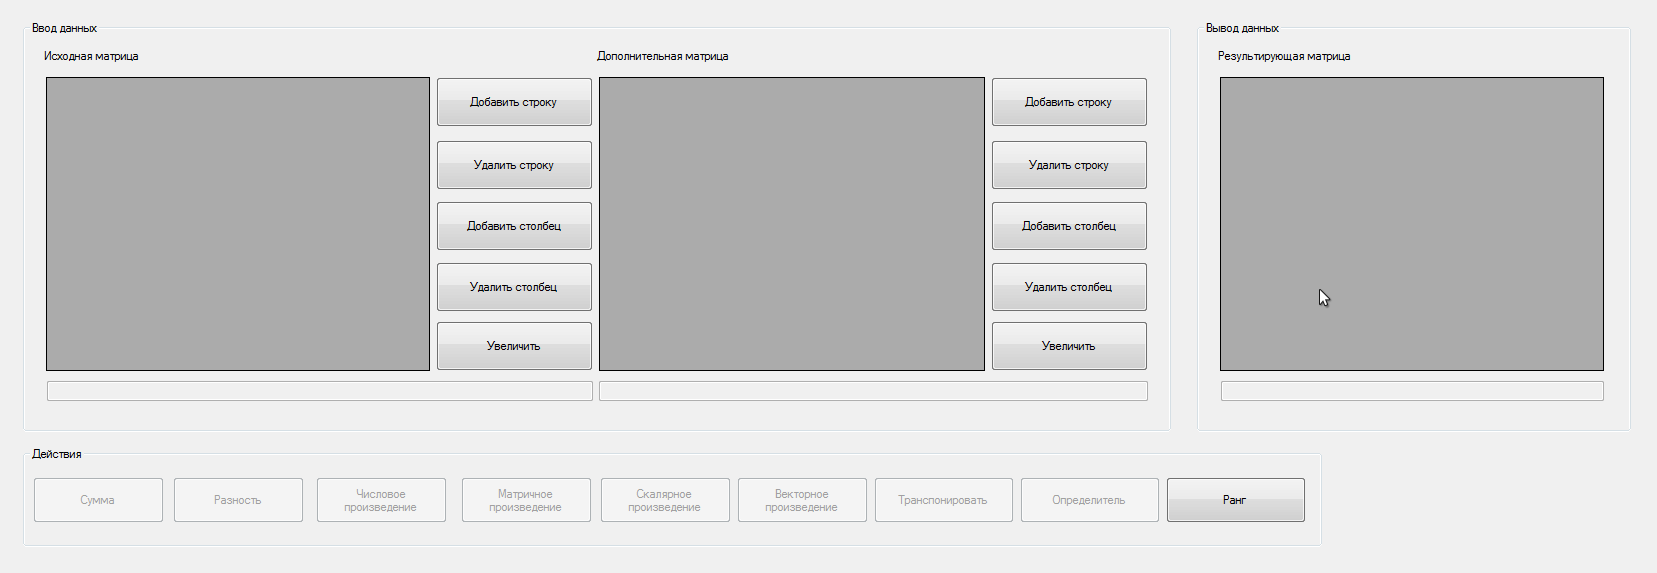
\includegraphics[width=0.5\linewidth]{images/matrix-calculator/form.png}
\caption{Форма окна для задания <<Простые вычисления>>}
\label{matrix-calculator-form}
\end{figure}

\subsection{Таблица с описанием элементов формы}
Все элементы формы были переименованы для большей читаемости. В таблице \ref{tab:matrix-calculator-form} представлены все изменения.


\begin{xltabular}{\textwidth}{| m{0.3\textwidth} | m{0.3\textwidth} | m{0.3\textwidth} |}

\hline
\textbf{Описание элементов формы} & \textbf{Список изменённых атрибутов} & \textbf{Новое значение атрибута} \\
\hline
\endfirsthead

\hline
\textbf{Описание элементов формы} & \textbf{Список изменённых атрибутов} & \textbf{Новое значение атрибута} \\
\hline
\endhead

\hline
\endfoot

\hline
\caption{Значение атрибутов элементов в матричном калькуляторе}
\label{tab:matrix-calculator-form}
\endlastfoot

Окно формы & Text & MatrixCalculator \\
Группа для ввода & Name & inputGroup \\
Группа для вывода & Name & outputGroup \\
Группа для действий & Name & actionsGroup \\
Метка для основной матрицы ввода & Name & initMatrixLabel \\
Метка для дополнительной матрицы ввода & Name & vectorLabel \\
Метка для матрицы вывода & Name & outputMatrixLabel \\
Таблица основной матрицы & Name & matrixInputInit \\
Таблица дополнительной матрицы & Name & matrixInputX \\
Таблица матрицы вывода & Name & matrixOutput \\
Поле ввода для вывода ошибок в исходной матрице & Name & inputInitErrorProvider \\
Поле ввода для вывода ошибок в дополнительной матрице & Name & inputXErrorProvider \\
Поле ввода для вывода ошибок в матрице вывода & Name & outputErrorProvider \\
Кнопка <<Добавить строку>> в исходную матрицу & Name & addRowInitButton \\
Кнопка <<Удалить строку>> в исходную матрицу & Name & rmRowInitButton \\
Кнопка <<Добавить столбец>> в исходную матрицу & Name & addColumnInitButton \\
Кнопка <<Удалить столбец>> в исходную матрицу & Name & rmColumnInitButton \\
Кнопка <<Увеличить>> в исходную матрицу & Name & addRowColumnInitButton \\
Кнопка <<Добавить строку>> в дополнительную матрицу & Name & addRowXButton \\
Кнопка <<Удалить строку>> в дополнительную матрицу & Name & rmRowXButton \\
Кнопка <<Добавить столбец>> в дополнительную матрицу & Name & addColumnXButton \\
Кнопка <<Удалить столбец>> в дополнительную матрицу & Name & rmColumnXButton \\
Кнопка <<Увеличить>> в дополнительную матрицу & Name & addRowColumnXButton \\
\end{xltabular}


\subsection{Примеры правильной и неправильной работы приложения}
При запуске приложения на экране появляется окно \ref{fig:matrix-calculator-start}.

\begin{figure}
\centering
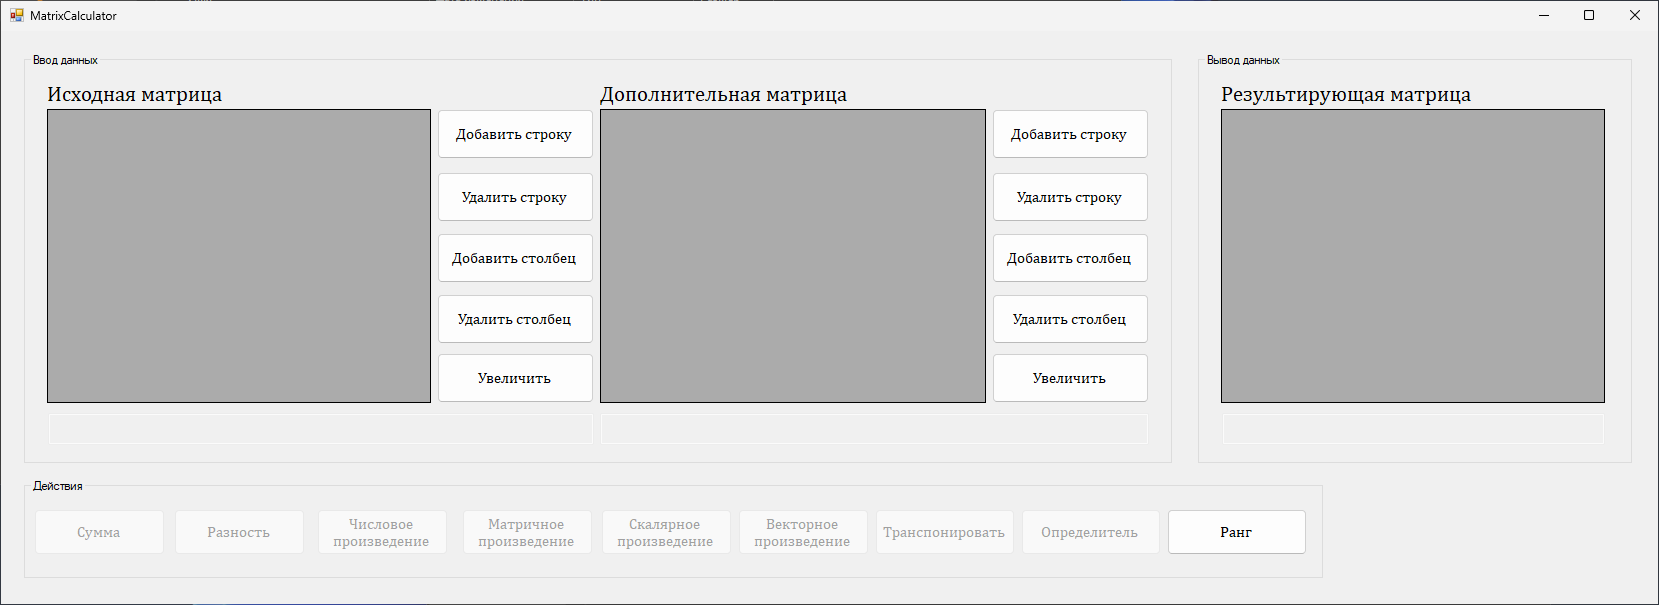
\includegraphics[width=0.5\linewidth]{images//matrix-calculator/start.png}
\caption{Запуск программы}
\label{fig:matrix-calculator-start}
\end{figure}

Кнопки активируются только тогда, когда операции над матрицами допустимы.\cite{patterny-oop} При нажатии на каждую кнопку происходит какое-то действие.

\begin{figure}
\centering
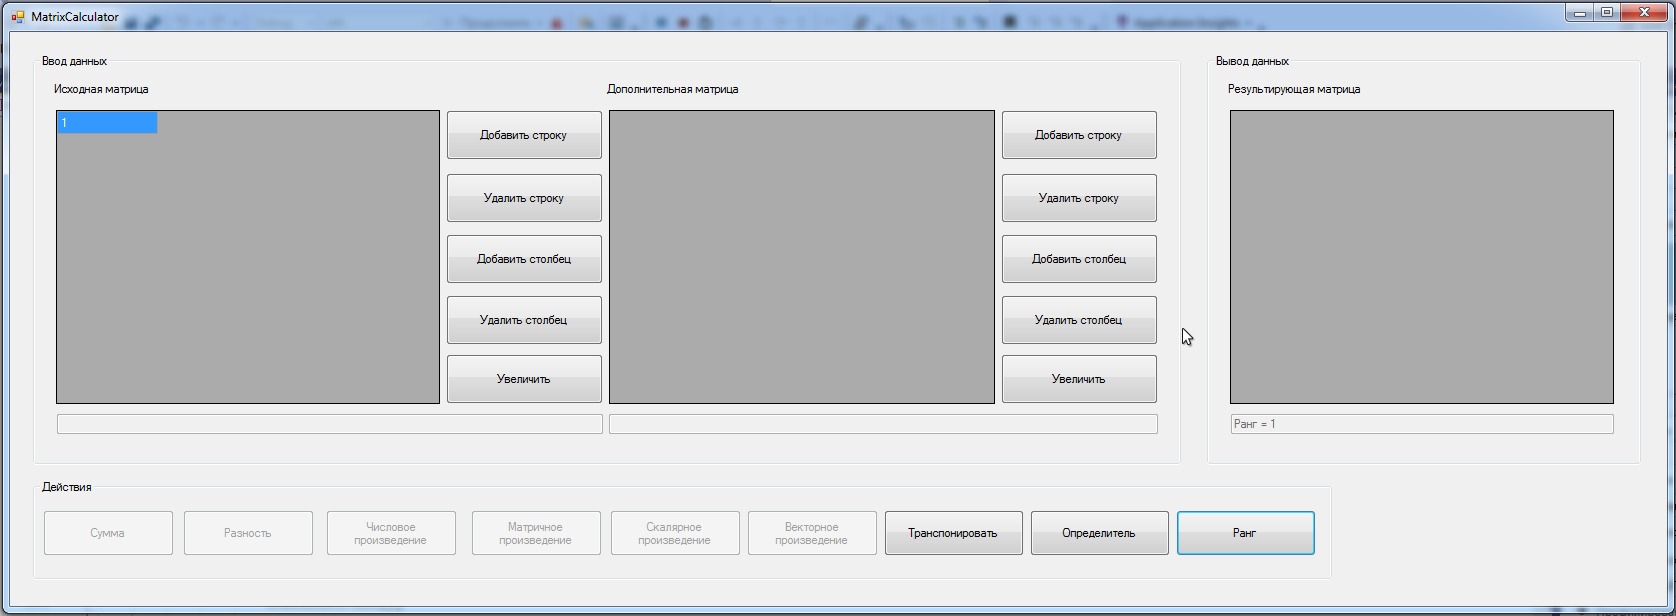
\includegraphics[width=0.5\linewidth]{images//matrix-calculator/okay.png}
\caption{Запуск с корректными данными}
\label{fig:matrix-calculator-okay}
\end{figure}

\begin{figure}
\centering
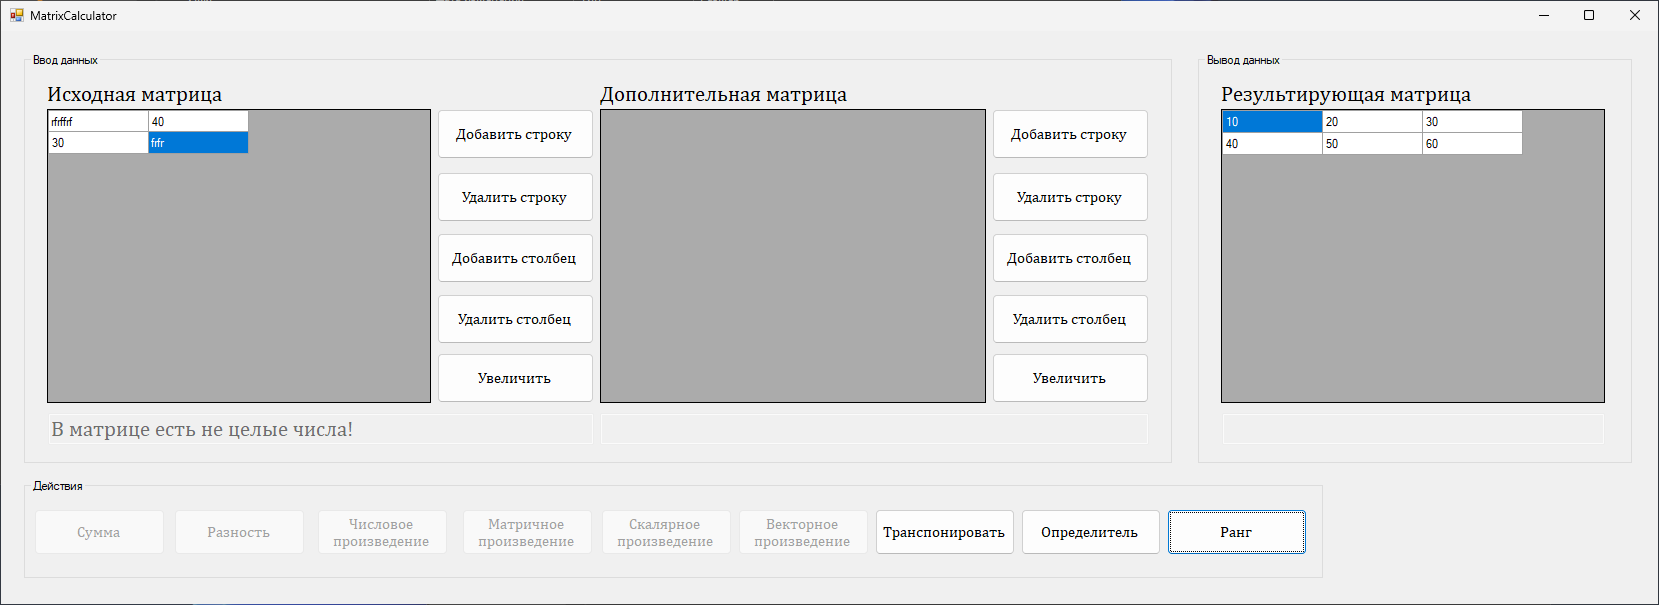
\includegraphics[width=0.5\linewidth]{images//matrix-calculator/error.png}
\caption{Пример ввода с некорректными данными}
\label{fig:matrix-calculator-error}
\end{figure}

\begin{figure}
\centering
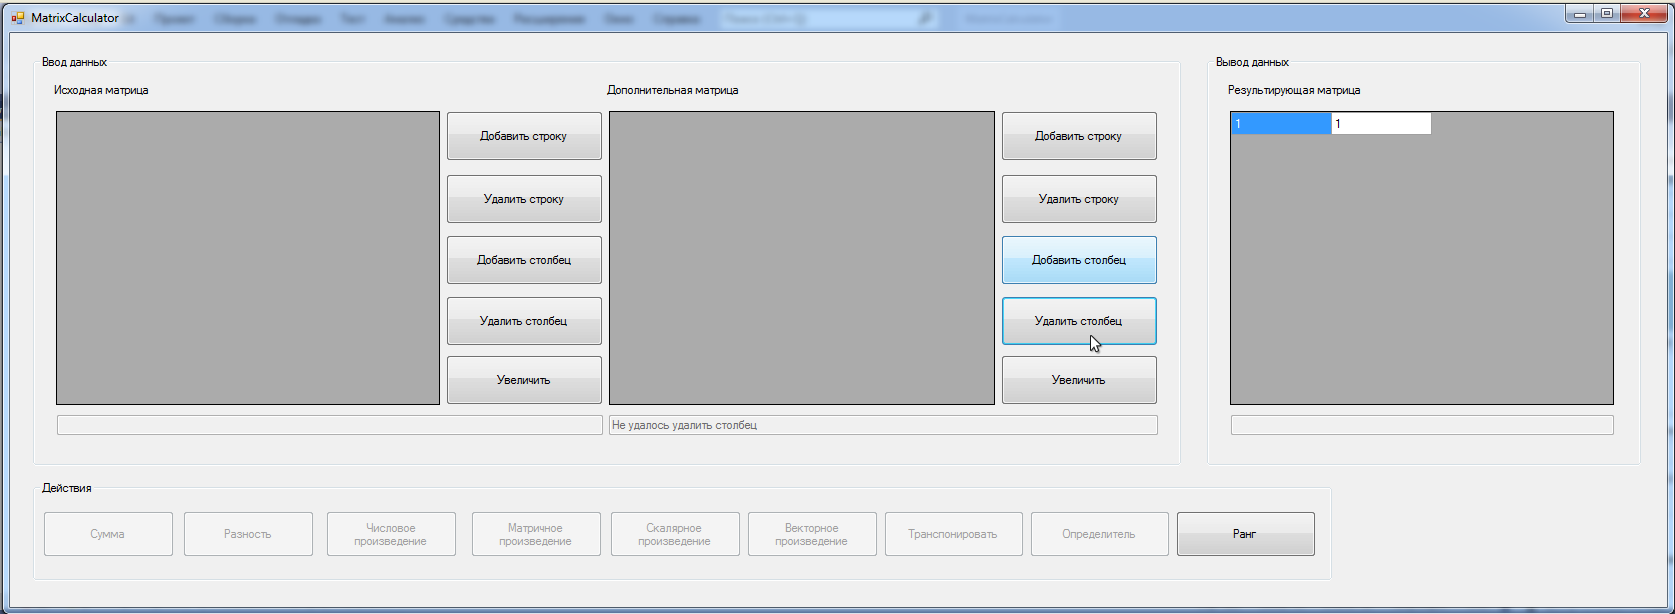
\includegraphics[width=0.5\linewidth]{images//matrix-calculator/error2.png}
\caption{Пример ввода с некорректными данными}
\label{fig:matrix-calculator-error2}
\end{figure}

\subsection{Примеры исходного кода}
\begin{minted}{cpp}
/* обработчик нажатия кнопки матричного произведения */
private: System::Void numericMultiplyButton_Click(System::Object^ sender, System::EventArgs^ e) {
    ClearAll();
    this->matrixOutput->RowCount = this->matrixInputInitial->RowCount;
    this->matrixOutput->ColumnCount = this->matrixInputInitial->ColumnCount;
    
    std::vector<std::vector<int>> matrixInitial;
    for (int i = 0; i < this->matrixInputInitial->RowCount; ++i) {
        std::vector<int> row;
        for (int j = 0; j < this->matrixInputInitial->ColumnCount; ++j) {
            int value;
            if (!Int32::TryParse(System::Convert::ToString(this->matrixInputInitial->Rows[matrixInputInitial->RowCount - i - 1]->Cells[j]->Value), value)) {
                this->inputInitialErrorProvider->Text = "В матрице есть не целые числа!";
                return;
            }
            row.push_back(value);
        }
    
        matrixInitial.push_back(row);
    }
    
    std::vector<std::vector<int>> matrixExtra;
    for (int i = 0; i < this->matrixInputExtra->RowCount; ++i) {
        std::vector<int> row;
        for (int j = 0; j < this->matrixInputExtra->ColumnCount; ++j) {
            int value;
            if (!Int32::TryParse(System::Convert::ToString(this->matrixInputExtra->Rows[matrixInputExtra->RowCount - i - 1]->Cells[j]->Value), value)) {
                this->inputExtraErrorProvider->Text = "В матрице есть не целые числа!";
                return;
            }
            row.push_back(value);
        }
    
        matrixExtra.push_back(row);
    }
    
    std::vector<std::vector<int>> matrixResult = multiplyMatrixByNumber(matrixInitial, matrixExtra[0][0]);
    
    for (int j = 0; j < this->matrixOutput->ColumnCount; ++j) {
        for (int i = 0; i < this->matrixOutput->RowCount; ++i) {
            this->matrixOutput->Rows[matrixInputInitial->RowCount - i - 1]->Cells[j]->Value = matrixResult[i][j];
        }
    }
}
\end{minted}

Больше кода проекта доступно в приложении \ref{application-A}. Также в приложенном архиве можно найти полный код проекта.

\conclusion

% Отобразить все источники. Даже те, на которые нет ссылок.
\nocite{*}

\bibliographystyle{ugost2003}
\bibliography{thesis}

% Окончание основного документа и начало приложений Каждая последующая секция
% документа будет являться приложением
\appendix

\end{document}
